% ReFind — Business Plan
% Build:  tectonic docs/business-plan.tex   (or: latexmk -pdf docs/business-plan.tex)
\documentclass[11pt,a4paper]{article}

\usepackage[margin=2.4cm]{geometry}
\usepackage[table]{xcolor}
\usepackage{titlesec}
\usepackage{enumitem}
\usepackage{booktabs}
\usepackage{amssymb}
\usepackage{tabularx}
\usepackage{array}
\usepackage{graphicx}
\usepackage{float}
\usepackage{tikz}
\usetikzlibrary{arrows.meta,positioning}
\usepackage{fancyhdr}
\usepackage{setspace}
\usepackage[hidelinks]{hyperref}

% ---------- Brand ----------
\definecolor{brand}{RGB}{13,115,119}      % ReFind teal
\definecolor{brandlight}{RGB}{232,242,242}
\definecolor{gris}{RGB}{90,98,102}

\titleformat{\section}
  {\Large\bfseries\sffamily\color{brand}}{\thesection.}{0.6em}{}
\titleformat{\subsection}
  {\large\bfseries\sffamily\color{brand!80!black}}{\thesubsection}{0.6em}{}
\titlespacing*{\section}{0pt}{18pt}{8pt}
\titlespacing*{\subsection}{0pt}{12pt}{5pt}

\setlength{\headheight}{22pt}
\pagestyle{fancy}
\fancyhf{}
\fancyhead[L]{\sffamily\small\color{gris}ReFind --- Business Plan}
\fancyhead[R]{\sffamily\small\color{gris}\thepage}
\renewcommand{\headrulewidth}{0.4pt}
\renewcommand{\headrule}{\hbox to\headwidth{\color{brand!40}\leaders\hrule height \headrulewidth\hfill}}

\newcolumntype{Y}{>{\raggedright\arraybackslash}X}

% Convenience environments
\usepackage{tcolorbox}
\newtcolorbox{highlight}{colback=brandlight,colframe=brand,boxrule=0.8pt,arc=2mm}

\setstretch{1.08}
\setlist{itemsep=2pt,topsep=4pt}

% ---------- Meta ----------
\newcommand{\TeamName}{Team ReFind}
\newcommand{\Semester}{Autumn 2026}

\begin{document}
\setcounter{tocdepth}{1}

% ================= COVER =================
\begin{titlepage}
\centering
\vspace*{1.2cm}
{\sffamily\color{brand}\rule{\textwidth}{1.5pt}}\\[6pt]
{\sffamily\Huge\bfseries\color{brand} ReFind}\\[10pt]
{\sffamily\LARGE Intelligent Lost \& Found, in Your Pocket}\\[8pt]
{\sffamily\large\color{gris} \textit{From lost to found --- automatically.}}\\[6pt]
{\sffamily\color{brand}\rule{\textwidth}{1.5pt}}\\[2.2cm]

{\sffamily\Large\bfseries App Business Plan}\\[0.4cm]
{\sffamily\large Mobile Intelligent Application --- Course Project}\\[2.4cm]

\renewcommand{\arraystretch}{1.5}
\begin{tabular}{>{\sffamily\bfseries}l l}
\toprule
Team & \TeamName \\
Semester & \Semester \\
\midrule
Members & Heng Liu --- Product \& Growth \\
        & Honghui Zhang --- Android Engineer \\
        & Yuchen Huang --- Backend \& AI Engineer \\
\bottomrule
\end{tabular}

\vfill
{\sffamily\small\color{gris}\Semester{} --- Confidential draft for coursework}
\end{titlepage}

\tableofcontents
\newpage

% ================= 1. EXECUTIVE SUMMARY =================
\section{Executive Summary}

Every year, a huge number of personal belongings --- phones, keys, ID cards, laptops, water
bottles, earbuds --- go missing on university campuses, in shopping centres, on public
transport, and at large events. Existing lost-and-found services are almost entirely
\textbf{passive}: the loser must search through piles of unclaimed items or scroll through
dozens of unrelated social-media posts, while the finder often has no practical way to reach
the owner. The result is a low return rate, frustrated users, and heavy manual workload for
campus security offices and service desks.

\textbf{ReFind} is a mobile application that turns lost-and-found from a searching problem
into a \textbf{matching problem}. A user who loses or finds an item simply uploads a photo
with the time and location. ReFind applies \textbf{image recognition and contextual
matching} (category, colour, location, time) to identify likely pairs automatically. When a
strong match is found, \textbf{both users are notified instantly}. To prevent false claims,
the claimed owner must pass a \textbf{private verification question} before any return is
arranged.

ReFind starts where the pain is most concentrated: \textbf{university campuses}, where users
are digitally native, density is high, and one institution can onboard thousands of users at
once. After proving the model on campuses, the same platform extends naturally to shopping
centres, public transport systems and large events --- any environment where items are lost
in high volume within a bounded area.

The business model is simple: the service is \textbf{free for individual users}, while
\textbf{organisations pay a subscription} for management dashboards, staff workflows and
data-analytics tools. Because matching is automated by machine learning, the marginal cost
of serving an additional campus is close to zero, and the social mission --- returning
people their belongings --- is also the product's growth engine: every successful return is
a word-of-mouth story.

\begin{highlight}
\textbf{Key facts.}
\begin{itemize}[leftmargin=1.2em,itemsep=2pt,topsep=3pt]
  \item \textbf{Product:} ReFind, an AI-powered lost-and-found app (Android first).
  \item \textbf{Users:} free for students and the general public.
  \item \textbf{Revenue:} B2B subscription from campuses, venues and transport operators,
        plus a merchant-sponsored reward pool.
  \item \textbf{Beachhead:} our own university campus, then city-wide institutions.
  \item \textbf{Core AI:} image-embedding matching + contextual filtering + LLM-generated
        verification questions.
  \item \textbf{Incentives:} owner-set rewards in escrow and merchant-sponsored points ---
        escrow and verification close the fraud and extortion levers. The platform never
        funds a reward itself.
\end{itemize}
\end{highlight}

% ================= 2. PROBLEM =================
\section{The Problem}

\subsection{Lost items rarely find their way home}

Losing a phone, wallet or student ID is not a trivial inconvenience: it interrupts study,
work and daily life, and replacement carries real cost. Yet the overwhelming majority of
lost items that \emph{are} found by someone never return to their owners, because the two
parties have no efficient way to meet.

\subsection{Current solutions are passive and fragmented}

\begin{itemize}
  \item \textbf{Lost-property offices and service desks} store found items, but they are
        passive warehouses: owners must actively call or visit, describe the item, and hope
        someone checks. There is no proactive notification, and coverage ends at the desk's
        opening hours.
  \item \textbf{Social media and group chats} (campus WeChat/QQ groups, WhatsApp groups,
        Facebook groups) carry lost-and-found posts, but they are unstructured: photos are
        buried in unrelated chatter, posts expire, and there is no matching at all --- a
        finder and a loser of the same umbrella can post in two different groups and never
        see each other.
  \item \textbf{Physical noticeboards} are even slower, with no photos, no search and no
        reach beyond one corridor.
\end{itemize}

\subsection{Three structural gaps}

\begin{enumerate}
  \item \textbf{No automatic matching.} Nobody connects ``lost'' and ``found'' reports of
        the same item; the burden of searching falls entirely on the person who already had
        the bad luck of losing something.
  \item \textbf{No trust layer.} Even when a channel works, anyone can claim anything:
        ``yes, that's my phone'' is unverifiable, so finders are rightly reluctant to hand
        items over.
  \item \textbf{No tools for organisations.} Campuses, malls and transport operators manage
        hundreds of items per month with spreadsheets and paper; they have no dashboard, no
        analytics and no API --- an unserved B2B need sitting right next to the consumer
        pain.
\end{enumerate}

% ================= 3. APP OVERVIEW =================
\section{App Overview: ReFind}

ReFind is a mobile app (Android first, iOS later) with two simple flows: \textbf{report} and
\textbf{claim}. Everything else --- matching, notification, verification --- is handled by
the platform. The complete loop has six steps (Figure~\ref{fig:flow}).

\begin{figure}[H]
\centering
\begin{tikzpicture}[
  font=\sffamily\small,
  stage/.style={draw=brand, fill=brandlight, thick, rounded corners=1.5mm,
               minimum width=3.5cm, minimum height=1.05cm, align=center},
  arr/.style={-{Stealth[length=2.5mm]}, thick, draw=brand!80},
  node distance=0.55cm and 0.7cm]
  \node[stage] (s1) {\textbf{1.} Photo report};
  \node[stage, right=of s1] (s2) {\textbf{2.} Auto matching};
  \node[stage, right=of s2] (s3) {\textbf{3.} Possible matches};
  \node[stage, below=0.7cm of s3] (s4) {\textbf{4.} Verification questions};
  \node[stage, left=of s4] (s5) {\textbf{5.} Chat \& handover};
  \node[stage, left=of s5] (s6) {\textbf{6.} Reward settlement};
  \draw[arr] (s1) -- (s2);
  \draw[arr] (s2) -- (s3);
  \draw[arr] (s3) -- (s4);
  \draw[arr] (s4) -- (s5);
  \draw[arr] (s5) -- (s6);
\end{tikzpicture}
\caption{The ReFind loop: from photo report to reward settlement. Every step is guarded
--- matching by confidence thresholds, claims by verification, rewards by escrow.}
\label{fig:flow}
\end{figure}

\subsection{Core user flows}

\begin{description}[style=nextline,leftmargin=1.2em]
  \item[Report.] The user uploads one or more photos, selects a category, and adds the time
        and location (auto-filled from GPS and the report timestamp, both editable). A short
        free-text description and optional private details (stickers, scratches, contents)
        complete the report in under a minute.
  \item[Automatic matching.] ReFind compares every new report against existing reports
        using image similarity and contextual signals. High-confidence pairs trigger
        \textbf{instant push notifications to both parties}; borderline pairs appear in a
        ``possible matches'' list for the user to review.
  \item[Verified claim.] When an owner contacts a finder, ReFind asks the owner
        item-specific verification questions generated from the \emph{private} details.
        Only after passing verification is the in-app chat opened, so the finder never
        hands a phone to a stranger who simply saw the post.
  \item[Optional reward.] When reporting, the owner may attach a reward --- set by the
        owner, \textbf{held in escrow by the platform}, and released to the finder only
        when both sides confirm the handover. Rewards settle as ReFind points redeemable
        for campus-merchant perks by default, with cash escrow for high-value items as a
        later phase (Section~\ref{sec:business-model}).
  \item[Return \& feedback.] Both sides confirm the handover and rate the interaction.
        Confirmed returns feed the matching system as positive training signal, build the
        finder's public ``good samaritan'' reputation, and release the escrowed reward;
        the organisation's dashboard records the item as resolved.
\end{description}

\subsection{Feature set at a glance}

\begin{itemize}
  \item \textbf{Photo-first reporting} with guided capture tips (sharp, well-lit,
        distinctive angle) to maximise match quality.
  \item \textbf{AI matching engine} combining image embeddings with category, colour, time
        and location filters (Section~\ref{sec:ai}).
  \item \textbf{Proactive notifications} --- the loser does not search; the system tells
        both sides when the same item appears.
  \item \textbf{Private verification questions} as an anti-fraud gate (Section~\ref{sec:ai}).
  \item \textbf{Incentive layer} --- optional owner-set rewards in escrow plus
        merchant-sponsored ReFind points, so returning an item is recognised concretely
        instead of relying on goodwill alone; every reward path is guarded by the
        anti-abuse controls in Section~\ref{sec:safety}.
  \item \textbf{In-app chat and handover confirmation} with safety guidance (meet at campus
        security points).
  \item \textbf{Organisation console (B2B):} item intake, storage location tracking, status
        workflow, expiry and disposal reminders, and return-rate analytics.
\end{itemize}

% ================= 4. AI =================
\section{How the Intelligence Works}
\label{sec:ai}

ReFind is, at its core, a \emph{mobile intelligent application}: the defensible part of the
product is the matching and verification pipeline, not the forms and feeds.

\subsection{Matching pipeline}

\begin{enumerate}
  \item \textbf{On-device image embedding.} Each uploaded photo is passed through a
        pre-trained vision model (CLIP-style image encoder, deployable on-device via
        TensorFlow Lite with a server-side fallback). The output is a normalised feature
        vector that captures the visual ``essence'' of the item --- shape, colour, texture
        --- independent of background and lighting.
  \item \textbf{Contextual filtering.} Candidate pairs are filtered by the structured
        signals users already provide: category, colour, a bounded time window, and a
        geographic radius around the reported location.
  \item \textbf{Composite score.} Final score $=$ cosine similarity of image embeddings
        combined with a weighted context score. Pairs above the auto-match threshold notify
        both users; pairs in a grey zone are surfaced as ``possible matches''; the rest are
        silently indexed.
  \item \textbf{Feedback loop.} Confirmed matches and confirmed non-matches tune the
        thresholds and weights per category (a laptop and a water bottle need different
        sensitivities).
\end{enumerate}

\subsection{LLM-generated verification questions}

When a claim is made, the system generates item-specific questions from the owner's
\emph{private} detail field (never shown publicly), e.g.\
\begin{itemize}
  \item ``What sticker is on the back of the laptop?''
  \item ``What is currently in the bottle's side pocket?''
  \item ``Is there any damage on the left corner? Describe it.''
\end{itemize}
The claimant must answer correctly before contact is unlocked. This single feature converts
ReFind from ``another noticeboard'' into a \emph{trusted} channel, and it is generated by an
LLM from the owner's own description --- zero manual configuration by staff.

\subsection{Privacy by design}
\label{sec:privacy}

Photos and locations are personal data. ReFind minimises by default: photos are visible only
to matched counterparties and (for organisations) staff; precise locations are blurred to a
zone-level for public display; reports auto-expire; and users can delete a report and all
associated data at any time, in line with GDPR and comparable personal-information
regulations.

% ================= 5. MARKET =================
\section{Market Analysis}

\subsection{Who feels the pain}

\begin{itemize}
  \item \textbf{Individuals:} every student and commuter is a potential user; losing an ID
        card, laptop or headphones is a near-universal experience.
  \item \textbf{Universities:} campus security and student-services desks accumulate
        hundreds of unclaimed items per term with manual, low-tech processes.
  \item \textbf{Venues and transport:} malls, stadiums, metro and bus operators publicly
        report tens to hundreds of thousands of lost items per year per network, and run
        dedicated departments to handle them.
\end{itemize}

\subsection{Beachhead: universities}

We deliberately start with universities because they combine all the conditions a two-sided,
local-network product needs:

\begin{itemize}
  \item \textbf{Density:} 10,000--30,000 users on one campus, losing items in the same
        buildings daily.
  \item \textbf{Homogeneity:} shared locations, shared terminology, one security office to
        partner with.
  \item \textbf{Digital-native users:} near-zero onboarding friction; students already live
        in campus-specific apps and group chats.
  \item \textbf{A natural champion:} the student union or campus security office can
        endorse the app and feed their existing stock of unclaimed items into it,
        instantly solving the two-sided cold-start problem from the supply side.
\end{itemize}

\subsection{Market sizing (estimates)}

\begin{table}[H]
\centering
\small
\renewcommand{\arraystretch}{1.35}
\begin{tabularx}{\textwidth}{l Y}
\toprule
\textbf{Layer} & \textbf{Definition and rough size} \\
\midrule
TAM & Digital lost-and-found for bounded venues (universities, malls, transit, events).
There are more than 160 higher-education institutions in the UK and over 3{,}000 in China
alone, plus thousands of large venues --- a global opportunity in the thousands of
potential B2B accounts. \\
SAM & Institutions in our launch regions that currently run a physical lost-property
operation and could adopt a managed digital platform within 3 years: estimated in the
hundreds of accounts. \\
SOM & Our 3-year target: 1 flagship campus pilot (year 1), 10 paying organisations
(year 2), 40 paying organisations (year 3). \\
\bottomrule
\end{tabularx}
\caption{Top-down market framing. All figures are planning estimates, to be refined with
pilot data.}
\end{table}

\subsection{Competition and positioning}

The market already has two clusters of incumbents, and naming them sharpens our position.
\textbf{B2B back-office software} --- Crowdfind and Chargerback (US venues and stadiums),
iLost (Europe) and Lost and Found Software (aviation and transit) --- digitises the
\emph{staff side}: intake, storage, claim web-forms and reporting for the counter that
holds the item. \textbf{AI matching platforms} are newer: Boomerang (US, venture-backed)
uses machine learning to match photos and descriptions of lost items for hotels, airports
and stadiums --- validating both the technology and institutional willingness to pay for
recovery. Both clusters, however, assume the item sits at an organisation's counter. None
of them operates a peer-to-peer network in which \emph{other students} are the finders ---
which is where most campus items actually are --- and none combines automatic matching
with a verification gate and an incentive layer in one consumer product.

\begin{table}[H]
\centering
\small
\renewcommand{\arraystretch}{1.3}
\begin{tabularx}{\textwidth}{>{\raggedright\arraybackslash}p{3.4cm} Y Y Y Y}
\toprule
 & \textbf{Auto-matching} & \textbf{Proactive notification} & \textbf{Anti-fraud verification} & \textbf{Org. tooling} \\
\midrule
Lost-property desks & -- & -- & partial & -- \\
Social media groups & -- & -- & -- & -- \\
Noticeboards & -- & -- & -- & -- \\
General marketplaces & -- & -- & -- & partial \\
B2B lost-property software (Crowdfind, Chargerback, iLost) & partial & partial & -- & \checkmark \\
AI matching apps (Boomerang) & \checkmark & partial & partial & \checkmark \\
\rowcolor{brandlight}
\textbf{ReFind} & \checkmark & \checkmark & \checkmark & \checkmark \\
\bottomrule
\end{tabularx}
\caption{Competitive comparison. \checkmark\ = full support; \emph{partial} = manual
review only, single scenario only, or no automatic notification; -- = not available.
Existing software digitises the back office or matches claims at a single venue's
counter; none combines a peer-to-peer consumer network with verification and incentives.}
\end{table}

\textbf{Strategic reading.} Boomerang's venture backing and growth validate that AI
matching works and that institutions pay for recovery. ReFind attacks the gap this wave
leaves open: the peer-to-peer campus network, where finders are students rather than
staff, gated by verification and motivated by escrowed rewards. Our moat is narrow but
real: the matching pipeline improves with local data (each campus's photos make its
matches better), network effects are local and fast to establish --- the first credible
app at one campus is hard to displace --- and the B2B console creates switching costs on
the institutional side.

% ================= USP =================
\section{Unique Selling Proposition}

\begin{highlight}
\textbf{USP.} ReFind is the only lost-and-found product built as a \emph{peer-to-peer
campus network}: it matches the photos of losers and finders automatically, verifies every
claim with questions only the true owner can answer, and rewards the return through
platform-escrowed incentives --- free for students, funded by institutions.
\end{highlight}

Three pillars back the statement:

\begin{enumerate}
  \item \textbf{Matching, not searching.} Every incumbent channel makes the unlucky
        person do the work. ReFind inverts this: the system watches all reports and tells
        both sides when the same item appears. B2B software (Section~5.4) digitises a
        counter; ReFind connects the campus population itself.
  \item \textbf{Trust engineered in, not bolted on.} LLM-generated verification questions
        and escrowed rewards are structural, not policies: a false claimant cannot pass
        the gate, and a hostage-taking finder has no lever. No competitor combines the
        two.
  \item \textbf{Aligned economics.} Students pay nothing, ever. Institutions pay because
        the platform measurably raises return rates and cuts desk workload. Merchants pay
        to appear at the moment of a happy return. Every side's incentive points the same
        way --- more verified returns.
\end{enumerate}

In one line for users: \textit{``Lose less. One photo, and the campus finds it back for
you.''} In one line for institutions: \textit{``Double your return rate without adding a
single desk hour.''} Both claims are falsifiable by the pilot (Section~\ref{sec:validation}),
which is the point.

% ================= PERSONAS =================
\section{Target User Personas}

ReFind serves two consumer roles and one institutional role. All three must be satisfied
for a single return to happen, so the product is designed against all three at once.

\begin{table}[H]
\centering
\footnotesize
\renewcommand{\arraystretch}{1.4}
\begin{tabularx}{\textwidth}{>{\sffamily\bfseries}p{1.7cm} Y Y Y}
\toprule
 & \textbf{Maya, 20} & \textbf{Daniel, 23} & \textbf{Officer Chen, 45} \\
 & undergraduate & postgrad teaching assistant & campus security supervisor \\
\midrule
Situation & Loses earbuds, student card or laptop at the library, gym or canteen; busy,
mobile-first, has posted to campus group chats before and got nothing back. & Often the
first to notice forgotten laptops and phones in teaching rooms; willing to help but has
no time to trek to the security desk and no safe way to hand items over. & Manages 300+
unclaimed items per term in spreadsheets; answers calls from anxious students and
parents; under pressure to raise the return rate with a fixed headcount. \\
Goals & Get the item back tonight, without begging in ten group chats. & Do the right
thing with one minute of effort --- and maybe a coffee for the trouble. & Higher return
rate, auditable records, less repetitive intake work. \\
Frustrations & Passive desks and unstructured group chats; no way to prove an item is
hers once someone answers. & Fear of scams or awkward negotiations with strangers;
uncertainty about liability. & Manual matching of claims to shelves; no data to justify
budget. \\
ReFind & 40-second report, automatic match notification, verified claim, handover
at a campus point she already passes. & One photo upload, auto-match does the finding,
escrowed reward settles instantly, handover witnessed at a staffed point. & Organisation
console: intake, storage tracking, claim moderation, return-rate analytics he can show
the administration. \\
\bottomrule
\end{tabularx}
\caption{Primary personas. Maya drives demand, Daniel drives supply, Officer Chen drives
adoption and pays.}
\end{table}

The campus context is what makes the triangle work: Maya and Daniel overlap physically
daily, and Officer Chen's endorsement removes the trust deficit a stranger-to-stranger
app would face.

% ================= BUSINESS MODEL =================
\section{Business Model}
\label{sec:business-model}

\subsection{Revenue streams}

\begin{description}[style=nextline,leftmargin=1.2em]
  \item[Free for individuals (forever).] Reporting, matching, notifications, verification
        and chat are free. This maximises adoption, which is the asset institutions pay
        for.
  \item[Organisation subscription (B2B SaaS).] Campuses, malls, transport operators and
        event organisers pay per site per year for the organisation console: staff
        workflows, storage tracking, moderated claims, branded app page, and analytics
        (return rate, hot-spot map, item-category trends, seasonal staffing hints).
  \item[Event packages (optional add-on).] Short-term deployments for conferences,
        festivals and stadiums: a branded instance live for the event duration.
  \item[Merchant-sponsored reward pool.] Campus caf\'es, bookstores and gyms sponsor
        ReFind points that finders redeem for real perks; sponsors get branded exposure
        inside the app and at the moment of a successful return --- the happiest moment a
        campus marketer can buy. This stream strengthens the incentive layer without
        touching consumer pricing: the platform never funds rewards, it only escrows and
        settles them.
\end{description}

\subsection{Indicative pricing}

\begin{table}[H]
\centering
\small
\renewcommand{\arraystretch}{1.3}
\begin{tabularx}{\textwidth}{l Y l}
\toprule
\textbf{Plan} & \textbf{What is included} & \textbf{Price (indicative)} \\
\midrule
Student / public & Full consumer app & Free \\
Campus & Console + analytics + moderation + support & \$2{,}500 / site / year \\
Large venue / transit & Multi-site, SSO, API, SLA & \$4{,}000--8{,}000 / year \\
Event & Branded temporary instance & \$300 / event \\
\bottomrule
\end{tabularx}
\caption{Pricing sketch for planning; to be validated in pilot negotiations.}
\end{table}

\subsection{Unit economics logic}

Serving one additional institution is almost pure margin: infrastructure cost is dominated
by photo storage and embedding inference, both of which cost fractions of a cent per report.
An LLM-generated verification question costs on the order of \$0.002 per claim. At pilot
scale (a few thousand reports per term per campus), the entire AI cost is negligible next
to one subscription cheque --- the constraint on growth is sales and onboarding, not
compute.

% ================= MARKETING =================
\section{Marketing Channels and Go-to-Market}
\label{sec:gtm}

\subsection{Marketing channels}

Channels are chosen against the personas (Section~7): each channel must reach either the
loser at the moment of loss, the finder at the moment of finding, or the institution that
controls adoption.

\begin{table}[H]
\centering
\small
\renewcommand{\arraystretch}{1.35}
\begin{tabularx}{\textwidth}{>{\raggedright\arraybackslash}p{3.6cm} l l Y}
\toprule
\textbf{Channel} & \textbf{Persona} & \textbf{Cost} & \textbf{Role in the funnel} \\
\midrule
Security-office partnership & Chen & Free & Endorsement, seed inventory of unclaimed
items, staffed handover points --- the trust foundation. \\
Student ambassador program & Maya, Daniel & \$500 / term & Peer credibility in faculties
and dorms; ambassadors seed the supply side among finders. \\
Loss-hotspot posters + QR & Maya & \$300 / term & Captured intent exactly where loss
happens (library, gym, canteen), at exam-season spikes. \\
Campus social media \& group chats & Maya, Daniel & Free & Awareness and launch bursts;
also our acquisition surface for the concierge validation (Section~\ref{sec:validation}). \\
Return stories (earned) & All & Free & Every verified return is shareable proof; with
consent, ``reunion'' posts become the growth loop. \\
\bottomrule
\end{tabularx}
\caption{Channel--persona--cost mapping for the campus phase.}
\end{table}

\subsection{Phase 1 --- Flagship campus pilot}

\begin{enumerate}
  \item \textbf{Partner first, launch second.} Sign the student union / campus security
        office as design partner. Their back catalogue of unclaimed items seeds the supply
        side on day one.
  \item \textbf{Campus ambassador program.} Recruit 10--20 student ambassadors across
        faculties and dorms; ambassadors get early access and swag, and run dorm-level
        demos.
  \item \textbf{Moment marketing.} Losses spike at exam season, orientation week and
        library closing time --- run ``Found something? One photo returns it.'' campaigns
        at those exact moments and locations (library, gym, canteen).
  \item \textbf{Let returns market the product.} Every successful return is a story: with
        user consent, share ``reunion'' posts on campus social channels. Return rate is our
        north-star metric and our best advertisement.
\end{enumerate}

\subsection{Phase 2 --- Replicate and convert}

Once one campus shows a measured return-rate uplift, the playbook repeats at 3--5 nearby
campuses. Institutions that actively use the console during the free pilot are converted to
paid subscriptions; the pilot contract includes a defined conversion point so the free
period is a sales process, not an open tab.

\subsection{Phase 3 --- Adjacent venues}

The same stack serves shopping centres, transit operators and events. We only enter these
after the campus playbook is documented, because each new vertical needs one dedicated
integration effort (e.g.\ transport operators need cross-city item routing).

% ================= 8. TECH =================
\section{Technical Feasibility}

\subsection{Architecture overview}

\begin{itemize}
  \item \textbf{Mobile client:} Android (Kotlin, Jetpack Compose) first; iOS later. Image
        embedding runs on-device via TensorFlow Lite where possible, with a server fallback
        --- good for latency, offline tolerance and privacy.
  \item \textbf{Backend:} REST API; PostgreSQL with the \texttt{pgvector} extension for
        similarity search; object storage for photos; push notifications via FCM.
  \item \textbf{AI services:} pre-trained CLIP-style encoder for embeddings (no model
        training required for MVP); perceptual hashing to suppress duplicate/re-uploaded
        photos; LLM API for verification-question generation and abuse filtering of report
        text.
\end{itemize}

\subsection{Why this is achievable}

Every AI component uses a \emph{pre-trained} model behind a stable API --- we are solving an
integration and product problem, not a research problem. The hardest engineering risks
(threshold calibration, false-positive fatigue) are addressed by the human-in-the-loop
``possible matches'' design: the system assists, the user decides, and every decision
improves the thresholds.

\subsection{Trust and safety engineering}
\label{sec:safety}

An incentive layer has two failure modes, and both are handled by design: with
\emph{no} incentive, the supply of returns dies because goodwill alone does not move
people to run errands for strangers; with an \emph{unguarded} incentive, bad actors arrive
--- false claimants, and finders who hold items hostage for more money. ReFind's controls:

\begin{itemize}
  \item \textbf{Escrow closes the extortion lever.} The reward is fixed by the owner and
        held by the platform before the handover is even arranged. A finder who demands
        ``extra cash or no phone'' gains nothing: the negotiated amount already exists,
        and off-platform demands are a reportable, bannable offence.
  \item \textbf{Verification closes the claim lever.} LLM-generated questions from private
        details (Section~4.2) gate every claim, and high-value categories (electronics,
        IDs) settle at staffed campus security points with an ID check.
  \item \textbf{Anomaly detection closes the farming lever.} Signals such as one account
        repeatedly ``finding'' high-value items, failed verification attempts, and
        report-rate spikes feed a moderation queue in the organisation console; confirmed
        fraud means suspension and, for theft, referral to campus security.
\end{itemize}

Report/claim abuse is additionally rate-limited and text-filtered. All personal data
handling follows data-minimisation and user-deletion rights (Section~\ref{sec:privacy}).

% ================= 9. ROADMAP =================
\section{Roadmap and Milestones}

\begin{table}[H]
\centering
\small
\renewcommand{\arraystretch}{1.35}
\begin{tabularx}{\textwidth}{l l Y}
\toprule
\textbf{Phase} & \textbf{Timing} & \textbf{Goals and exit criteria} \\
\midrule
M1 --- Design & Months 1--2 & Requirements, UI prototypes, matching-pipeline spike on
sample photos. Exit: clickable prototype + offline matching demo. \\
M2 --- MVP & Months 3--5 & Android app: report, browse, image + context matching,
notifications. Exit: end-to-end match found in test set. \\
M3 --- Trust layer & Months 6--7 & Verification questions, escrowed rewards, in-app chat,
organisation console v1. Exit: full return flow completed in beta. \\
M4 --- Campus pilot & Month 8+ & Flagship campus live with security office; measure
return rate vs.\ baseline. Exit: agreed pilot KPI met. \\
M5 --- Commercialise & Year 2 & Convert pilot to paid; onboard 10 organisations; begin
iOS client. Exit: first recurring revenue. \\
\bottomrule
\end{tabularx}
\caption{Product and commercial roadmap.}
\end{table}

% ================= FINANCIALS =================
\section{Financial Overview and Key Metrics}

\subsection{Cost structure}

\begin{table}[H]
\centering
\small
\renewcommand{\arraystretch}{1.3}
\begin{tabularx}{\textwidth}{l Y l}
\toprule
\textbf{Item} & \textbf{Notes} & \textbf{Year-1 estimate} \\
\midrule
Cloud \& storage & App server, PostgreSQL, photo storage & \$1{,}200 \\
AI inference & Embeddings + LLM verification at pilot scale & \$500 \\
App distribution & Developer program fees & \$125 \\
Pilot marketing & Ambassadors, print, launch events & \$1{,}000 \\
Contingency & --- & \$500 \\
\midrule
\textbf{Total} & & \textbf{\$\textasciitilde4{,}000} \\
\bottomrule
\end{tabularx}
\caption{Year-1 operating cost at pilot scale. Development labour is excluded (student
project; for a funded venture this becomes the dominant line).}
\end{table}

\subsection{Revenue projection}

\begin{table}[H]
\centering
\small
\renewcommand{\arraystretch}{1.3}
\begin{tabularx}{\textwidth}{l Y Y Y}
\toprule
 & \textbf{Year 1} & \textbf{Year 2} & \textbf{Year 3} \\
\midrule
Paying organisations & 0 (free pilots) & 10 & 40 \\
Avg.\ subscription & --- & \$2{,}500 & \$3{,}200 \\
\textbf{Revenue} & \textbf{\$0} & \textbf{\$25{,}000} & \textbf{\$\textasciitilde130{,}000} \\
Operating cost & \$4{,}000 & \$12{,}000 & \$45{,}000 \\
\textbf{Net} & \textbf{--\$4{,}000} & \textbf{+\$13{,}000} & \textbf{+\$\textasciitilde85{,}000} \\
\bottomrule
\end{tabularx}
\caption{Three-year planning projection. Break-even occurs during Year 2 with the first
subscription cohort.}
\end{table}

The projection is intentionally conservative: it assumes revenue comes only from B2B
subscriptions and ignores event packages and any consumer monetisation. The strategic point
is that the model reaches break-even at a scale (10 organisations) that is reachable by
direct campus-to-campus sales, without requiring mass consumer monetisation.

\subsection{Key metrics}

The plan is managed by a small set of metrics with explicit targets; each one can kill or
confirm an assumption in this document.

\begin{table}[H]
\centering
\small
\renewcommand{\arraystretch}{1.35}
\begin{tabularx}{\textwidth}{>{\raggedright\arraybackslash}p{4.4cm} l Y}
\toprule
\textbf{Metric} & \textbf{Pilot target} & \textbf{Why it matters} \\
\midrule
Verified returns / month (north star) & 150 by end of campus pilot & Returns are the
product; every other metric is a proxy for this one. \\
Auto-match precision & $\geq$80\% of notifications are true pairs & False-match
notifications destroy trust faster than missed matches lose returns. \\
D7 retention (closed beta) & $\geq$25\% & Losing things is episodic; retention must come
from the network's ongoing value, not one user's bad luck. \\
Median time-to-return & $<$48 hours & The headline number for all marketing claims and
the institutional sales pitch. \\
Pilot $\rightarrow$ paid conversion & $\geq$40\% of active pilots & Validates that free
pilots are a sales pipeline, not charity. \\
Gross margin & $>$85\% & Confirms the near-zero-marginal-cost SaaS assumption behind
Section~8. \\
\bottomrule
\end{tabularx}
\caption{Key metrics with pilot-phase targets.}
\end{table}

% ================= VALIDATION =================
\section{Channels to Validate the App}
\label{sec:validation}

Before and alongside the MVP build, four validation channels are used, ordered from
cheapest to most expensive, each with a falsifiable success criterion:

\begin{enumerate}
  \item \textbf{Landing page + waitlist.} A one-page pitch with campus social posts
        driving traffic, sign-up open before the app exists. \emph{Criterion:} at least
        8\% of visitors join the waitlist.
  \item \textbf{Concierge MVP in campus groups.} For two weeks the team manually matches
        lost and found posts in existing group chats with a shared spreadsheet and the
        matching heuristics. \emph{Criterion:} at least 5 verified returns complete
        end-to-end, and participants agree to move to the app when it ships.
  \item \textbf{Instrumented closed beta.} Fifty students on the full MVP.
        \emph{Criteria:} D7 retention $\geq$25\%, at least 60\% of reports receive a
        candidate match within 24 hours, auto-match precision stays $\geq$80\%.
  \item \textbf{Pilot KPI review with the security office.} Measured return-rate uplift
        against the pre-app baseline plus staff hours saved per week. \emph{Criterion:}
        the uplift converts the office into the first paying organisation
        (Section~\ref{sec:gtm}, Phase 2).
\end{enumerate}

Each channel de-risks a different layer --- demand, matching quality, retention, and
willingness to pay --- so a failure pinpoints the broken assumption instead of sinking
the project.

% ================= RISKS =================
\section{Risk Analysis}

\begin{table}[H]
\centering
\small
\renewcommand{\arraystretch}{1.35}
\begin{tabularx}{\textwidth}{>{\raggedright\arraybackslash}p{3.6cm} l Y}
\toprule
\textbf{Risk} & \textbf{Level} & \textbf{Mitigation} \\
\midrule
Two-sided cold start & High & Seed supply side via campus security office's existing item
stock; launch in one dense campus, not city-wide. \\
False claims / fraud & Medium & LLM verification questions, claim audit log, escalation to
staff for high-value items. \\
Reward abuse (hostage pricing, theft-for-reward) & Medium & Fixed escrowed rewards remove
the negotiation lever; security-point settlement with ID checks; anomaly detection on
repeat high-value finds; suspension and referral. \\
Privacy / data protection & Medium & Data minimisation, zone-level locations, auto-expiry,
one-tap deletion; GDPR-aligned design. \\
Matching quality below expectation & Medium & Human-in-the-loop ``possible matches'',
per-category thresholds, feedback loop; on-device embedding with server fallback. \\
Low institutional willingness to pay & Medium & Free pilot with defined conversion point;
lead with measured return-rate uplift and staff-time savings. \\
Incumbent copying & Low & Local data moat, institution lock-in via console and analytics. \\
\bottomrule
\end{tabularx}
\caption{Key risks and mitigations.}
\end{table}

% ================= 12. TEAM =================
\section{Team}

\begin{table}[H]
\centering
\small
\renewcommand{\arraystretch}{1.4}
\begin{tabularx}{\textwidth}{l Y}
\toprule
\textbf{Member} & \textbf{Role and responsibility} \\
\midrule
Heng Liu & Product \& growth --- requirements, business model, pilot partnerships; also
design system, campus ambassador program and pilot metrics. \\
Honghui Zhang & Android engineer --- app architecture and on-device ML integration;
TensorFlow Lite embeddings and client-side performance. \\
Yuchen Huang & Backend \& AI engineer --- matching service, verification pipeline and
data layer; pgvector similarity search and LLM integration. \\
\bottomrule
\end{tabularx}
\caption{Team roles and responsibilities.}
\end{table}

\vspace{6pt}
\noindent\textbf{Concluding note.} ReFind takes a problem everyone has personally
experienced, replaces passive searching with proactive AI matching, and attaches a clean
B2B revenue model to a free consumer service. The beachhead is one campus we can walk to,
the technology is pre-trained and proven, and every successful return makes both the
network and the model stronger.

\end{document}
